\chapter{Thermal Hydraulics}
\label{ch:thermalHydraulics}

\section{Introduction}
  Material temperatures are a pivotal part of the multi-physics problem of
  simulating a Fast Reactor (FR). Temperatures are necessary for
  calculating reactor cross-sections for an accurate power distribution and can
  be used as input for a thermal hydraulic simulation. Thermal hydraulic models
  are developed for standard FR geometry as described in
  \sref{sec:geometry_description}. Recall, the standard assembly is a hexagonal 
  can and filled with many cylindrical rods. 

  In this simulation, two thermal hydraulic models are employed. The first is a 
  steady-state, one-dimensional, axial heat convection model to calculate coolant 
  temperatures and densities as the coolant flows vertically through a channel.
  This model is valid for the assumption of no cross-flow between channels and 
  perfect fluid mixing within the flow channel. These assumptions are valid for
  simulating fast reactors with canned assemblies and assembly designs which 
  encourage within-assembly mixing. Hexagonal assemblies as common to FRs and 
  described in \sref{sec:geometry_description} satisfy this assumption with 
  canned assemblies to prevent cross-flow between channels and mixing encouraged
  by wire wrapping. The second model is a radial steady-state, one-dimensional,
  radial heat conduction model within a cylindrical rod to calculate average 
  cladding, bond, and fuel temperatures.

  \begin{figure}
    \centering
    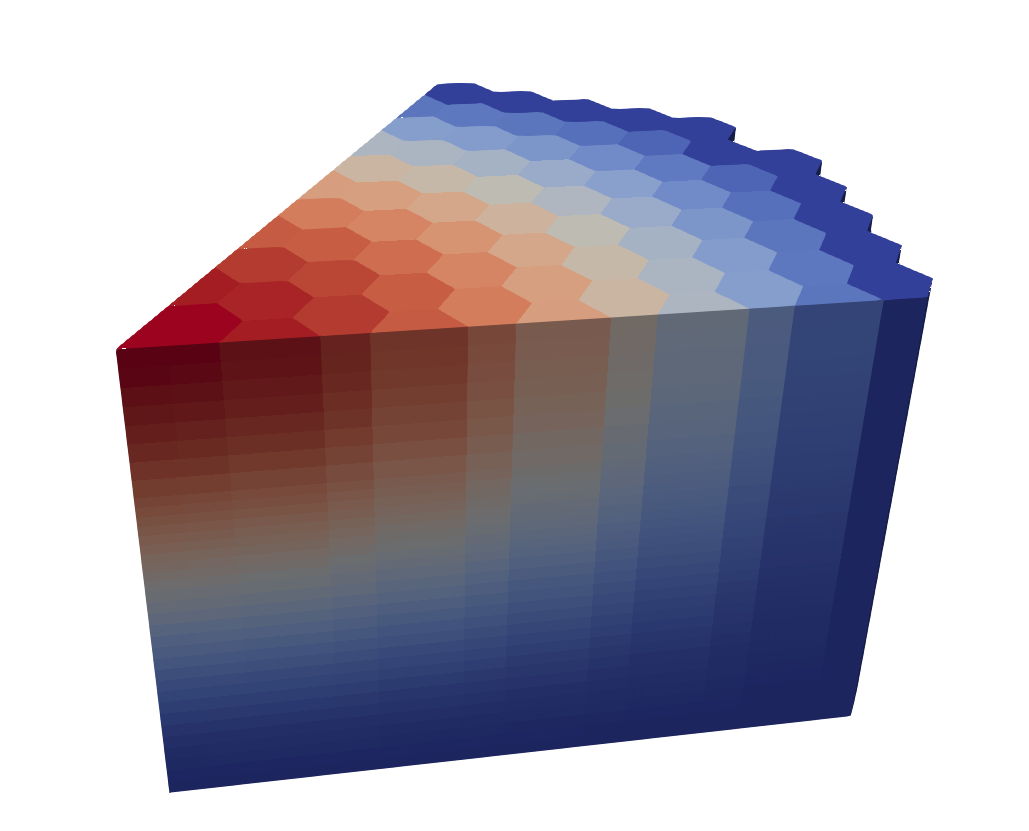
\includegraphics[width=\textwidth]{enthalpy_rise}
    \caption{Typical FR Enthalpy Rise.}
    \label{fig:enthalpy_rise}
  \end{figure}

\section{Material Properties}
  \label{sec:material_properties}
  Thermodynamic properties of reactor materials are required for these models.
  The coolant properties are the most extensive with density, enthalpy, 
  thermal conductivity, dynamic viscosity, and heat capacity required. In this
  thesis, sodium coolant is considered. However, these thermal hydraulic
  properties can be easily changed to allow for the simulation of fast reactors
  with other coolants such as lead or molten salt. The 
  functional forms of sodium thermal hydaraulic properties are given in 
  \cite{sodiumProp}. 
  Thermal conductivity values are also required for the cladding and fuel
  material. Typical cladding for fast reactor designs is HT9 stainless-steel and
  a functional form of the thermal conductivity is given in \cite{ht9Prop}. Both
  sodium and steel have relatively high thermal conductivities and their thermal
  conductivities do not change significantly over the operating temperatures of
  SFRs. Therefore, the thermal conductivity of sodium within the bond and HT9 
  are assumed constant at the average value as reported in \cite{sodiumProp} and
  \cite{ht9Prop} respectively. These constant values are given in 
  \tref{tab:constant_k}.
    
  \begin{table}
    \caption{Constant Thermal Conductivity for Sodium and HT9.}
    \label{tab:constant_k}
    \begin{center}
      \begin{tabular}{cl}
        \toprule
        Material & $k \units{$\frac{\text{W}}{\text{m K}}$}$ \\
        \midrule
        Sodium &  64.33 \\
        HT9    &  25.81 \\
        \bottomrule
      \end{tabular}
    \end{center}
  \end{table}

  Fuel composition is assumed to be of the form U-XZr where
  X is the weight fraction of Zr in the fuel. A typical value for X is 10\%.
  A fuel thermal conductivity given in \cite{fuelProp} as a function of material
  temperature and zirconium weight fraction.
  A plot of thermal conductivity for U-10Zr as a function of temperature is 
  given in \fref{fig:kfuel_plot}. For the expression of fuel thermal 
  conductivity cited, the integral of thermal conductivity is unbounded as 
  $T \rightarrow 0$ so thermal conductivity is assumed constant below 300 
  \units{K} which is below the melting point of sodium so this assumption is 
  valid for sodium-cooled reactor applications.

  \begin{figure}
    \centering
    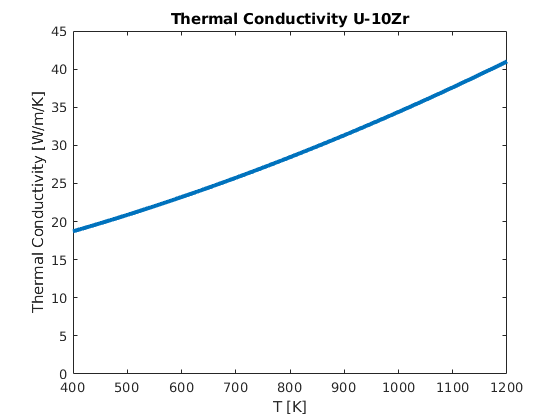
\includegraphics[width=0.7\textwidth]{kfuel_plot}
    \caption{Variable Thermal Conductivity in Fuel.}
    \label{fig:kfuel_plot}
  \end{figure}

\section{Power Normalization}
  Recall the multigroup neutron diffusion equation solved via the power
  iteration method returns the largest eigenvalue $\keff$ and unique positive
  eigenvector $\phi_g$ (see \sref{sec:power_iterations}). The neutron flux
  calculated according to this method is an eigenvector and can be normalized
  to an arbitrary constant. For a specified total reactor power, $Q_{Rx}$ the
  normalization constant can be calculated. For un-normalized neutron flux as
  calculated by the power iteration method, $\widetilde{\phi_{g,e}}$, for  
  energy group $g$ in finite element $e$, the normalization constant is 
  \begin{equation}
    \label{eq:normalization_c}
    c = \frac{Q_{Rx}}{\sum_{g}^{G} \sum_{e}^{N_E} \kappa \Sigma_{f,g,e} \,
      \widetilde{\phi_{g,e}} \, V_e}
  \end{equation}
  where $c$ is the normalization constant and $V_e$ is the volume of element
  $e$. $\kappa$ represents the reclaimable (non-neutrino) energy produced per
  fission such that the quantity $\kappa \Sigma_f \phi$ represents the
  volumetric heat generation rate. 
  %Similar to $\nu\Sigma_{f,g}$, $\kappa\Sigma_{f,g}$ is 
  %calculated as an aggregate quantity and not simply $(\kappa)(\Sigma_{f,g})$.
  Then the properly scaled neutron flux is given as
  \begin{equation}
    \label{eq:normalization_phi}
    \phi_{g,e} = c \, \widetilde{\phi_{g,e}}
  \end{equation}
  and the total power generated in each element is 
  \begin{equation}
    \label{eq:elementpwr}
    q_{e} = \sum_g^G \kappa \Sigma_{f,e,g} \, \phi_{g,e} \, V_e .
  \end{equation}
  The quantity $q_e$ has units \units{W}. Assuming all heat generated in the
  element is generated within the fuel, the volumetric heat generation rate 
  within the fuel is 
  \begin{equation}
    \label{eq:elementqppp_fuel}
    q'''_{e} = \frac{q_e}{V_{fuel,e}}
  \end{equation}
  where $V_{fuel,e}$ is the volume of fuel in element $e$. The quantity $q'''_e$
  has units \units{$\frac{\text{W}}{\text{m}^3}$} and will be necessary for the 
  radial conduction model.

\section{Axial Convection Model}
  \label{sec:axial_convection_model}
  In this model, the temperature and density of the coolant is calculated as
  it flows upward through a single hexagonal assembly.

  \subsection{Geometric Model}
    Used in association with an unstructured mesh, the thermal hydraulic model
    requires mapping mesh elements into reactor assemblies. In the input
    geometry file, the user must specify to which one-dimensional flow channel 
    each element belongs.
    Adopting the nomenclature from fast reactors, each flow channel represents a
    hexagonal assembly. In the following discussion, an assemlby index is
    subscripted $i$ for $i = 1,2,\ldots,N_{hex}$ where $N_{hex}$ is the number
    of hexagonal assemblies in the simulated reactor. 

    The concept of ``chunks'' is also introduced for use in the discretization 
    of the thermal hydraulic model. A chunk is the set of all elements in a 
    channel with a unique axial elevation. For example, in a fast reactor 
    hexagonal assembly, the assembly has a unique $i$ index and contains a 
    number of chunks equal to the number of axial elevations in the simulation. 
    Additionally, each chunk is required to have unique material composition. 
    The relationship of elements, chunks, and hexes is shown in 
    \fref{fig:chunk_description}. Chunks are indexed $j = 1,2,\ldots,N_C$ where
    $N_C$ is the total number of chunks.  For $N_z$ axial elevations, 
    $N_C = N_{hex} \, N_z$. The indexing of chunks is chosen such that 
    $j+N_{hex}$ is the chunk one axial elevation above chunk $j$. The alignment
    of chunks in a one-dimensional flow channel is shown in
    \fref{fig:axial_model}.

    \begin{figure}
      \centering
      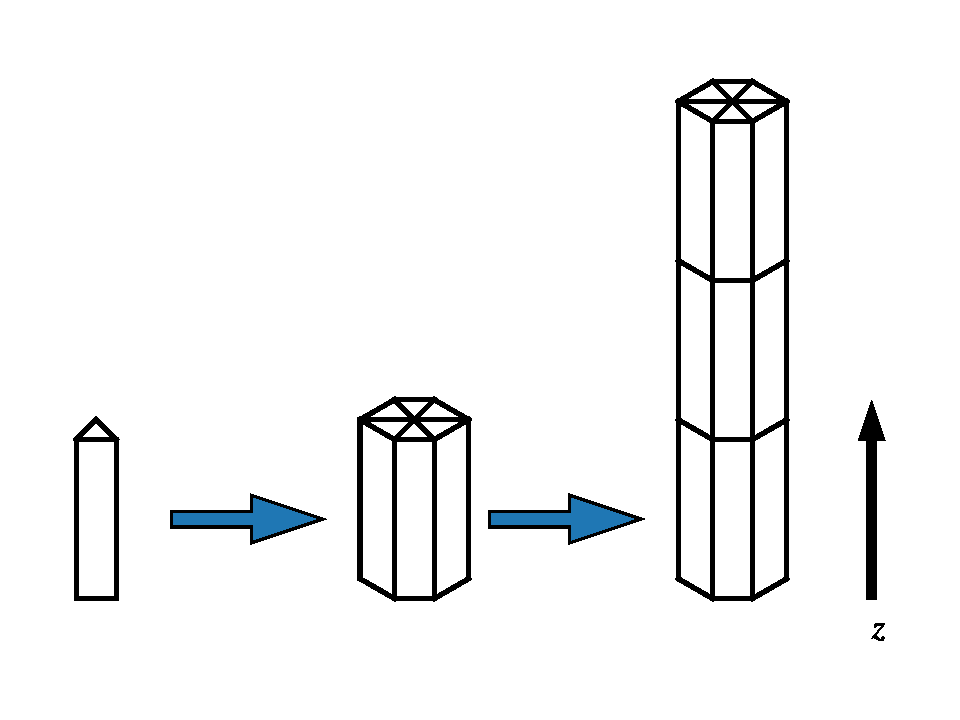
\includegraphics[width=0.7\textwidth]{chunk_description}
      \caption{Progression of Element (left), to Chunk (center), to Hex 
        (right).}
      \label{fig:chunk_description}
    \end{figure}
    
    \begin{figure}
      \centering
      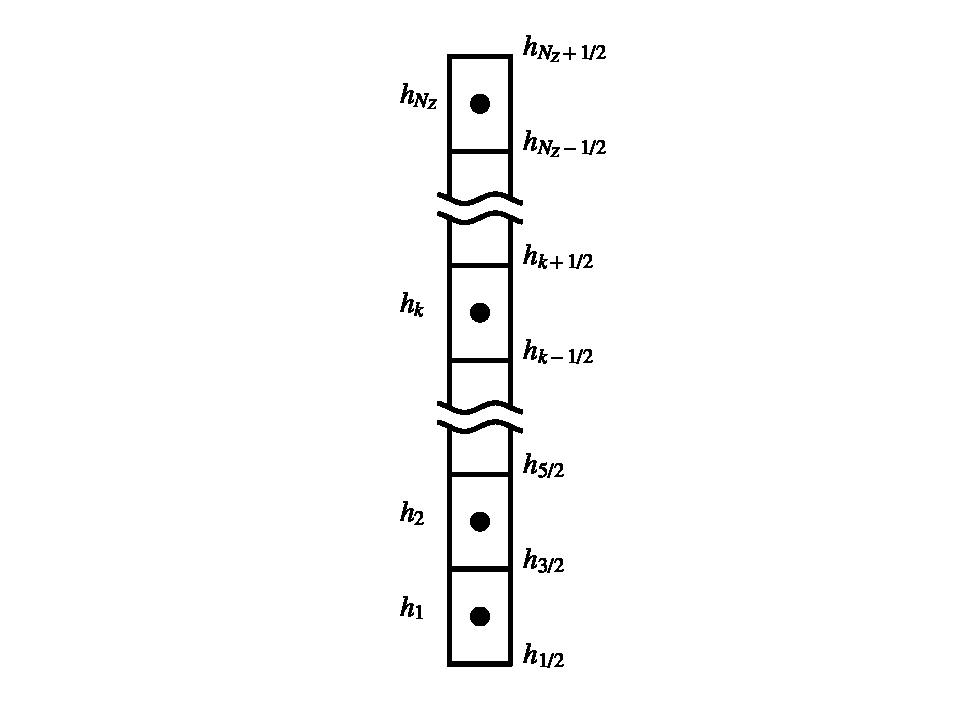
\includegraphics[width=0.2\textwidth]{axial_model}
      \caption{One-Dimensional Axial Heat Convection Model Description.}
      \label{fig:axial_model}
    \end{figure}

  \subsection{Channel Mass Flow}
    The channel mass flow, $\mdot_i$, must be calculated given a user 
    specified total reactor mass flow rate $\mdot_{Rx}$.  Mass flow is 
    partitioned into each channel assuming constant mass flux at the reactor 
    inlet according to 
    \begin{equation}
      \label{eq:mass_flow_split}
      \mdot_i = \mdot_{Rx} \frac{A_{cool,i}}{A_{cool,Rx}}
    \end{equation}
    where $A_{cool,i}$ is the coolant flow area for channel $i$, $N_{rod,i}$ is
    the number of rods within the assembly $i$, and $A_{cool,Rx}$
    is the coolant flow area for the reactor.  The mass flow per unit area is 
    assumed constant at the reactor inlet and the mass flow in a channel is the
    product of the mass flux and the channel flow area. This partitioning of
    mass flow rate is chosen to allow for assemblies with different flow areas
    or the modeling of partial assemblies in fractional core models.

  \subsection{Chunk Powers}
    For the one-dimensional heat convection model in the axial direction,
    heat generation quantities are needed for chunks. Heat generation quantities
    for elements are calculated in \eref{eq:elementpwr} and
    \eref{eq:elementqppp_fuel}.
    For the axial heat convection model, the total heat generated in a chunk,
    $q_j$, and the average volumetric heat generation rate in the fuel for
    elements within the chunk, $q'''_j$. 
    These relationships are given in \eref{eq:chunkpwr} and
    \eref{eq:chunkqppp_fuel} respectively. The notation $e \in j$ implies the
    summation over all elements $e$ within chunk $j$.
    \begin{align}
      \label{eq:chunkpwr}
      q_j &= \sum_{e \in j} q_e \\
      \label{eq:chunkqppp_fuel}
      q'''_j &= \frac{\sum_{e \in j} q'''_e V_{fuel,e}}{\sum_{e \in j} 
        V_{fuel,e}}
    \end{align}
  
  \subsection{Channel Enthalpy}
    It is assumed that all heat generated within the chunk is deposited in the
    coolant as it flows through the chunk. This occurs at steady-state. Then, 
    the steady-state coolant enthalpy for an axial location $z$ within the 
    channel is expressed by a simple energy balance relation as
    \begin{equation}
      \label{eq:continuous_heat_balance}
      h_i(z) = h_{in} + \frac{1}{\mdot_i} \int_0^z q'_i(z') \; dz'
    \end{equation}
    where $h_i(z)$ is the specific enthalpy at axial position $z$ in channel 
    $i$, $h_{in}$ is the inlet enthalpy, $\mdot_i$ is the mass flow rate within
    the channel given in \eref{eq:mass_flow_split}, and 
    $q'_i(z)$ is the linear heat generation rate for channel $i$ at elevation 
    $z$. $h_{in}$ is related to a user specified coolant inlet temperature,
    $T_{inlet}$, by a state relationship for the coolant 
    $h_{in} = h(T_{inlet})$.  

    The integral in \eref{eq:continuous_heat_balance} can be discretized along
    the channel and converted to a summation. In this discretization, the model
    in \fref{fig:axial_model} is used where $h_{j+1/2}$ is the enthalpy at the
    upper edge of the chunk and $h_j$ is the average enthalpy within the chunk.
    Then, the discretization of the integral \eref{eq:continuous_heat_balance}
    is 
    \begin{equation}
      \label{eq:heat_balance}
      h_{j+1/2} = 
        h_{in} + \frac{1}{\mdot_i} \sum_{k=1}^{N_z} q'_{j} \, \Delta z_{j}
    \end{equation}
    where $q'_{j}$ is the linear heat generation rate in the chunk $j$ in
    channel $i$ and ${\Delta z_{j} = z_{j+1} - z_{j}}$. 
    (Note: by indexing properly, $j = i + (k-1) \, N_{hex}$.)
    Recognizing the quantity $q_{j} = q'_{j} \Delta z_{j}$
    is the total heat generated in chunk $j$, then \eref{eq:heat_balance} can 
    be rewritten.
    \begin{equation}
      h_{j+1/2} = h_{in} + \frac{1}{\mdot_i} \sum_{k=1}^{N_z} q_{i,k}
    \end{equation}
    The quantity $h_{j+1/2}$ represents the enthalpy in channel $i$ at the upper 
    coordinate of the one-dimensional heat convection chunk (see
    \fref{fig:axial_model}). The node-average enthalpy is instead desired. To 
    first-order approximation, then
    \begin{equation}
      h_j = \half (h_{i,k-1/2}+h_{i,k+1/2})
    \end{equation}
    where $h_j$ is the average enthalpy in chunk $j$ located in channel $i$ at
    axial level $k$.
    The final result of this model is $h_j$, the bulk coolant enthalpy in each
    chunk $j$. Given, $h_j$, the average bulk coolant temperature in the chunk
    $T_{\infty,j} = T(h_j)$ can be calculated using a state relationship in
    \cite{sodiumProp}. Bulk coolant temperature will be an input into the Radial
    Conduction Model, \sref{sec:radial_conduction_model}, to later calculate
    temperatures in the fuel rod.
  
\section{Radial Conduction Model}
  \label{sec:radial_conduction_model}
  The radial heat conduction model calculates the steady-state heat
  conduction from its generation in the fuel to the coolant. This model
  represents an average fuel rod in each fuel bundle. The model explicitly
  treats fuel, sodium bond, and cladding regions.
  In the radial heat conduction model, it is assumed that all heat generated in
  the reactor is due directly to fission as described by the volumetric heat
  generation rate ${q'''=\kappa \Sigma_f \phi}$. However, other sources of heat
  also contribute to reactor power. Gamma radiation can account for up to 14\%
  of heat generated throughout the core. Additionally, via beta deposition and
  elastic neutron scattering, roughly 2\% of fission energy is deposited in the
  cladding material \cite{FastSpectrumReactors}.
  
  For this model, it is assumed
  that the bulk coolant temperature, $T_{\infty,j}$, is known within the chunk 
  as calculated in \sref{sec:axial_convection_model}. Then, the model begins by 
  calculating temperatures at key locations. Material temperature is calculated
  at the fuel center-line, fuel surface, bond surface, and clad surface. The
  derivation of these quantities are presented in \sref{sec:surface_temps}. 
  Similar results can be found in \cite{FastSpectrumReactors}. With the
  temperatures at these locations calculated, the average temperature within
  each material is calculated. These average temperatures are essential for the
  accurate simulation of the reactor as they influence multigroup constants.

  \subsection{Geometric Model}
    For the purposes of the radial model, geometry is described in
    \fref{fig:radial_model}. This model represents a cylindrical fuel pellet,
    surrounded by sodium bond, enclosed in steel cladding, with sodium coolant
    flowing in the axial direction. The center of the fuel rod is located at
    $r=0$ where $r$ is the radial coordinate. The fuel pellet has radius $R_F$
    and fuel is located in $r \in [0,R_F)$. Then, bond is located in 
    $r \in (R_F,R_B)$ and clad is located in $r \in (R_B,R_C]$. The fuel 
    center-line temperature is $T_0$ and fuel surface temperature is $T_F$. Bond
    surface temperature is $T_B$ and clad surface temperature is 
    $T_C$. $T_{\infty}$ represents the bulk coolant temperature. In this model,
    heat is generated exclusively in the fuel with volumetric heat generation 
    rate $q'''$. 

    \begin{figure}
      \centering
      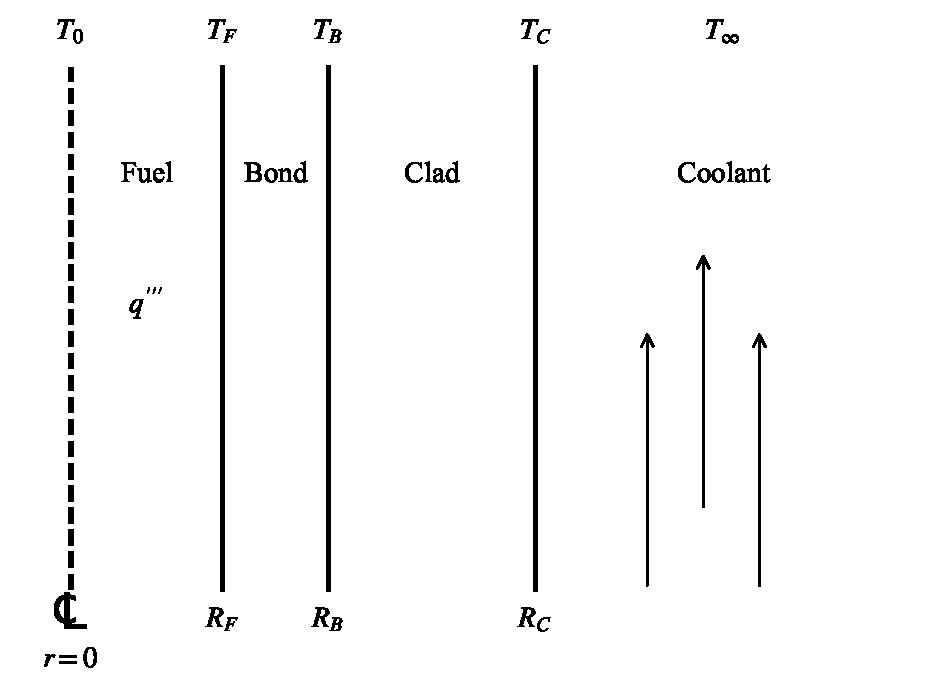
\includegraphics[width=0.5\textwidth]{radial_model}
      \caption{Geometry Description of Radial Heat Conduction Model.}
      \label{fig:radial_model}
    \end{figure}

  \subsection{Surface Temperature and Center-Line Temperatures}
    \label{sec:surface_temps}
    Temperatures at selected locations are calculated using the steady-state
    heat conduction equation with material properties described in
    \sref{sec:material_properties}. The process of the derivation moves outward
    from the fuel center-line toward the coolant flow, always assuming that the
    next surface temperature is known. Derivation begins with the fuel 
    center-line temperature, assuming the fuel surface temperature is known. 
    Then, derivation moves to the fuel surface temperature assuming the bond 
    surface temperature is known. This pattern is terminated and the 
    relationship is closed at the cladding surface where, for a given 
    $T_{\infty}$ the clad surface temperature is described by Newton's law of 
    cooling and a convective heat transfer correlation. For this work, the 
    Weisman correlation is selected for its applicability to triangular-pitch 
    flow channels \cite{weisman}.

    With derivation completed, the temperatures of interest are calculated.
    While derivation moved from fuel center-line outward to clad surface,
    calculation moves from clad surface inward to fuel center-line. This is
    necessary because the quantities are all unknown with the exception of
    $T_{\infty}$ so the calculation begins there. Surface temperatures are all
    described explicitly due to the assumption of constant thermal conductivity
    within bond and clad regions. Fuel center-line temperature must be solved
    implicitly due to the treatment of variable thermal conductivity. A
    numerical solution method is used to solve for the fuel center-line
    temperature.
    
    \subsubsection{Temperature in Fuel}
      The fueled region is the only region modeled with non-zero volumetric heat
      generation. In this region, $q'''_j$ as specified by 
      \eref{eq:chunkqppp_fuel} is assumed constant within the fuel. 
      Additionally, the thermal conductivity in the fuel will be assumed to have
      general form $k_F(T)$. For this work, $k_F(T)$ is specified by the
      functional form from \cite{fuelProp}. For the assumed fuel composition, 
      the thermal conductivity is plotted in \fref{fig:kfuel_plot}.

      The steady-state heat conduction equation with constant volumetric heat
      generation rate $q'''_j$ and variable thermal conductivity $k_F(T)$ can be
      written.
      \begin{equation}
        \label{eq:conduction_fuel}
        \grad \cdot (k_F(T_F(r)) \grad T_F(r)) + q'''_j = 0
      \end{equation}
      Noting the gradient operator in one-dimensional cylindrical geometry,
      \eref{eq:conduction_fuel} is rewritten with partial derivatives.
      \begin{equation}
        \label{eq:conduction_fuel_cylindrical}
        \frac{1}{r} \frac{\partial}{\partial r} \left( r \, k_F(T_F(r)) \, 
          \frac{d \, T_F}{dr} \right) + q'''_j = 0
      \end{equation}
      Note the inner derivative is an ordinary derivative because the only
      function to which it applies, $T_F(r)$, is a function of one variable. The
      outer derivative is a partial derivative because it applies to $T_F(r)$ as
      well as $k_F(T_F(r))$.

      Begin solving \eref{eq:conduction_fuel_cylindrical} by multiplying the
      equation by radial coordinate $r$.
      \begin{equation}
        \frac{\partial}{\partial r} \left( r\, k_F(T_F(r)) \, \frac{d\, T_F}{dr} 
        \right) + q'''_j = 0
      \end{equation}
      Integrate the equation for $r \in [0,r']$ where $r'$ is an arbitrary
      location $r' \in [0,R_F]$.
      \begin{align}
        \int_0^{r'} \left( \frac{\partial}{\partial r} \left( r\, k_F(T_F(r)) \, 
          \frac{d\, T_F}{dr} \right) + q'''_j \right) \; dr &= 0 \\
        \int_0^{r'} \frac{\partial}{\partial r} \left( r\, k_F(T_F(r)) 
          \frac{d \, T_F}{dr} \right) \; dr + \int_0^{r'} q'''_j \; dr &= 0 \\
        \label{eq:need_bc}
        \left[ r \, k_F(T_F(r)) \frac{d\,T_F}{dr} \right]_{r=0}^{r=r'} + 
          \left. \frac{q'''_j}{2} r^2 \right|_{r=0}^{r=r'} &= 0 \\
      \end{align}
      Using a symmetry boundary condition at $r=0$, then 
      \begin{equation}
        \left. \frac{d \, T_F}{dr} \right|_{r=0} = 0
      \end{equation}
      and \eref{eq:need_bc} can be evaluated.
      \begin{equation}
        \label{eq:dtdr_fuel}
        \left. r' k_F(T_F(r')) \frac{d\,T_F}{dr} \right|_{r=r'} + 
          \frac{q'''_j}{2} r^{\prime 2} = 0
      \end{equation}
      Divide by the location $r'$.
      \begin{equation}
        \left. k_F(T_F(r')) \frac{d \, T_F}{dr}\right|_{r=r'} + 
          \frac{q'''_j}{2} r' = 0
      \end{equation}
      Next, integrate $r' \in [0,r]$.
      \begin{align}
        \int_0^r \left( k_F(T_F(r')) \left. \frac{d\,T_F}{dr}\right|_{r=r'} 
          + \frac{q'''_j}{2} r' \right) \; dr' &= 0 \\
        \int_0^r k_F(T_F(r')) \left. \frac{d\,T_F}{dr}\right|_{r=r'} \; dr' + 
          \int_0^r \frac{q'''_j}{2} r' \; dr' &= 0 \\
        \int_0^r k_F(T_F(r')) \left. \frac{d\,T_F}{dr}\right|_{r=r'} \; dr' + 
          \left. \frac{q'''_j}{4} r^{\prime 2} \right|_{r'=0}^{r'=r} &= 0 \\
        \int_0^r k_F(T_F(r')) \left. \frac{d\,T_F}{dr}\right|_{r=r'} \; dr' + 
          \frac{q'''_j}{4} r^2 &= 0
      \end{align}
      The fundamental theorem of calculus allows for the expression of the first
      integral.
      \begin{equation}
        \label{eq:tcl_integral}
        \int_{T_F(0)}^{T_F(r)} k_F(T_F(r)) \; dr + \frac{q'''_j}{4} r^2 = 0
      \end{equation}
      In this derivation, $k_F(T)$ is allowed to be a generic function. 
      Therefore, \eref{eq:tcl_integral} does not have a simple forward 
      expression. Solving for $T_F(0)$ will require a non-linear search such as
      the bisection method. Define the conductivity integral of the fuel
      conductivity in the form as
      \begin{equation}
        \label{eq:conductivity_integral}
        K_F(T) = \int_0^T k_F(T') \; dT'
      \end{equation}
      where $k_F(T)$ is the thermal conductivity of the fuel material as shown
      in \fref{fig:kfuel_plot}. Then, \eref{eq:tcl_integral} can be rewritten.
      \begin{gather}
        K_F(T_F(r)) - K_F(T_F(0)) + \frac{q'''_j}{4} r^2 = 0 \\
        \label{eq:tfuel_r}
        K_F(T_F(0)) = K_F(T_F(r)) + \frac{q'''_j}{4} r^2 \\
        \label{eq:tcl_conductivity_integral}
        K_F(T_F(0)) = K_F(T_F) + \frac{q'''_j}{4} R_F^2
      \end{gather}
      The fuel center-line temperature can be calculated using
      \eref{eq:tcl_conductivity_integral} given a functional form of the
      conductivity integral $K_F(T)$ by performing a search on the function
      where $T_F(0)$ is the fuel center-line temperature, $T_F=T_F(R_F)$ is the
      fuel surface temperature, and $R_F$ is the radius of the fuel.
      If, instead, $k_F(T)$ were constant such that $k_F(T) = k_F$, then
      \eref{eq:tcl_conductivity_integral} would be equivalent to 
      \begin{align}
        \label{eq:tfr}
        T_F(r) &= T_F(0) - \frac{q'''_g}{4 \overline{k_F}} r^2 \\
        \label{eq:tcl_constant_kfuel}
        T_F(0) &= T_F + \frac{q'''_j}{4 \overline{k_F}} R_F^2
      \end{align}
      where $\overline{k_F}$ is the effective thermal conductivity in the fuel
      region.
      To calculate $T_F(0)$, the fuel surface temperature must be known.
      If more information is known about $K_F(T)$, a forward expression
      may be possible. However, a bisection method is implemented to maintain
      generality.

    \subsubsection{Temperature in Sodium Bond}
      The fuel surface temperature is calculated by considering the heat
      conduction equation in the sodium bond region. There is no heat generation
      in this region so $q'''=0$. 
      The thermal conductivity in the bond is assumed constant such that 
      ${k_B(T) = k_B = 64.33 \units{$\frac{\text{W}}{\text{m K}}$}}$ as 
      specified in \tref{tab:constant_k}.
      The steady-state heat conduction equation with no heat generation is
      written as
      \begin{equation}
        \label{eq:tc_grad}
        \grad \cdot (k_B \grad T_B(r)) = 0
      \end{equation}
      where $k_B$ is a constant representing the thermal conductivity of the
      sodium in the bond. $k_B = 64.33 \units{$\frac{\text{W}}{\text{m K}}$}$ as
      specified in \tref{tab:constant_k}.
      $T_B(r)$ is the temperature within the bond region.
      In this region, good thermal contact between the fuel and bond is
      assumed such that
      \begin{equation}
        \label{eq:rf_temp_continuity}
        T_F(R_F)=T_B(R_F).
      \end{equation}
      That is, the temperature is 
      continuous at the material discontinuity. Additionally, constant heat flux
      is assumed at the material discontinuity such that
      \begin{equation}
        \label{eq:rf_flux_continuity}
        k_F(T_F(R_F)) \left.\frac{d\,T_F}{dr}\right|_{r=R_F} = 
          k_B \left.\frac{d\,T_B}{dr}\right|_{r=R_F}.
      \end{equation}

      Recognizing one-dimensional cylindrical geometry, \eref{eq:tc_grad} can 
      be rewritten.
      \begin{equation}
        \label{eq:tb_heat_conduction}
        \frac{1}{r} \frac{d}{dr} \left( r \, k_B \frac{d \, T_B}{dr} \right) = 0
      \end{equation}
      Begin solving \eref{eq:tb_heat_conduction} by multiplying the equation by
      the radial coordinate $r$.
      \begin{equation}
        \frac{d}{dr} \left( r \, k_B \frac{d \, T_B}{dr} \right) = 0
      \end{equation}
      Integrate the equation for $r \in[R_F,r']$ where $r'$ is an arbitrary
      location $r' \in [R_F,R_B]$.
      \begin{align}
        \int_{R_F}^{r'} \frac{d}{dr} \left( r\, k_B \, 
          \frac{d\,T_B}{dr} \right) \; dr &= 0\\
        \left. r\, k_B \frac{d\,T_B}{dr} \right|_{r=R_F}^{r=r'} &= 0 \\
        \label{eq:tf_first_integral}
        \left. r' \, k_B \frac{d\,T_B}{dr} \right|_{r=r'} - 
          \left. R_F \, k_B \frac{d\,T_B}{dr} \right|_{r=R_F} &= 0
      \end{align}
      The assumption of constant heat flux at the material boundary given in 
      \eref{eq:rf_flux_continuity} allows for the treatment of the spatial 
      derivative at $R_F$. Recall from the derivation within the fuel region, 
      the expression \eref{eq:dtdr_fuel} is exploited. The expression is valid 
      for any $r' \in [0,R_F]$ so allow $r'=R_F$.
      \begin{align}
        \left. R_F k_F(T_F(R_F)) \frac{d\,T_F}{dr} \right|_{r=R_F} + 
          \frac{q'''_j}{2} R_F^2 &= 0 \\
        \label{eq:surface_relation}
        \left. R_F k_F(T_F(R_F)) \frac{d\,T_F}{dr} \right|_{r=R_F} &= 
          - \frac{q'''_j}{2} R_F^2
      \end{align}
      Recall from the earlier derivation of the fuel center-line temperature 
      that the quantity $q'''_j$ is the average volumetric heat generation rate
      within chunk $j$ specified in \eref{eq:chunkqppp_fuel}.
      \eref{eq:surface_relation} is substituted into
      \eref{eq:tf_first_integral}.
      \begin{equation}
        \label{eq:tf_first_bc}
        \left. r' \, k_B \frac{d\,T_B}{dr} \right|_{r=r'} +
          \frac{q'''_j}{2} R_F^2 = 0
      \end{equation}
      Divide \eref{eq:tf_first_integral} by the radial coordinate $r'$. This is
      valid because $r' \ne 0$ in this region.
      \begin{equation}
        \left. k_B \frac{d\,T_B}{dr} \right|_{r=r'} + 
          \frac{q'''_j}{2} \frac{R_F^2}{r'} = 0
      \end{equation}
      Integrate the equation for $r' \in [R_F,r]$ where $r \in [R_F,r']$.
      \begin{align}
        \int_{R_F}^r \left( \left. k_B \frac{d\,T_B}{dr}\right|_{r=r'}
          + \frac{q'''_j}{2} \frac{R_F^2}{r'} \right) \; dr' &= 0 \\
        \int_{R_F}^r \left. k_B \frac{d\,T_B}{dr}\right|_{r=r'} \; dr'
          + \int_{R_F}^r \frac{q'''_j}{2} \frac{R_F^2}{r'} \; dr' &= 0\\
        k_B \int_{R_F}^r \left. \frac{d\,T_B}{dr}\right|_{r=r'} \; dr'
          + \frac{q'''_j}{2} R_F^2 \left. \ln(r') \right|_{r'=R_F}^{r'=r} &= 0\\
        k_B \int_{R_F}^r \left. \frac{d\,T_B}{dr}\right|_{r=r'} \; dr'
          + \frac{q'''_j}{2} R_F^2 ( \ln(r) - \ln(R_F)) &= 0 \\
        k_B \int_{R_F}^r \left. \frac{d\,T_B}{dr}\right|_{r=r'} \; dr'
          + \frac{q'''_j}{2} R_F^2 \ln\left(\frac{r}{R_F}\right) &= 0 
      \end{align}
      Again, the remaining integral can be rewritten by employing the
      fundamental theorem of calculus.
      \begin{equation}
        \label{eq:tf_fundamental_theorem}
        k_B (T_B(r) - T_B(R_F)) + \frac{q'''_j}{2} R_F^2 
          \ln\left(\frac{r}{R_F}\right) = 0
      \end{equation}
      Then, solving for $T_B(R_F)$.
      \begin{align}
        \label{eq:tbr}
        T_B(r) &= T_B(R_F) - \frac{q'''_j}{2 k_B} R_F^2 
          \ln\left(\frac{r}{R_F}\right) \\
        \label{eq:tf_forward}
        T_B(R_F) &= T_B(R_B) + \frac{q'''_j}{2 k_B} R_F^2 
          \ln\left(\frac{R_B}{R_F}\right)
      \end{align}
      The fuel surface temperature can be calculated using
      \eref{eq:tf_forward} for constant thermal conductivity $k_B$.
      In \eref{eq:tf_forward}, the bond surface temperature must be
      given to calculate the fuel surface temperature.

    \subsubsection{Temperature in Cladding}
      Consider the heat conduction equation in the cladding region. Derivation
      of the bond surface temperature $T_B=T_B(R_B)$ is similar to
      the fuel surface temperature because both consider a heat conduction
      equation with no heat generation and constant thermal conductivity.
      The
      thermal conductivity in the clad is assumed constant such that $k_C(T) =
      k_C = 25.81 \units{$\frac{\text{W}}{\text{m K}}$}$ as specified in
      \tref{tab:constant_k}.
      Using the expression for temperature within the bond,
      \eref{eq:tf_forward}, the temperature within the cladding can be expressed
      similarly by changing material subscripts. 
      \begin{align}
        \label{eq:tcr}
        T_C(r) &= T_C(R_B) - \frac{q'''_j}{2 k_C} R_F^2
          \ln\left(\frac{r}{R_B}\right) \\
        \label{eq:tb_forward}
        T_C(R_B) &= T_C(R_C) + \frac{q'''_j}{2 k_C} R_F^2
          \ln\left(\frac{R_C}{R_B}\right)
      \end{align}
      The bond surface temperature can be calculated using \eref{eq:tb_forward}
      for constant thermal conductivity $k_C$. In \eref{eq:tb_forward}, the clad
      surface temperature must be given to calculate the bond surface
      temperature.

    \subsubsection{Clad Surface Temperature}
      Clad surface temperature $T_C$ is given by Newton's Law of Cooling with
      convective heat transfer coefficient $H$ specified according to the
      Weisman correlation \cite{weisman}. Newton's Law of Cooling may be written 
      as
      \begin{equation}
        q''_{clad} = H_c (T_C - T_{\infty})
      \end{equation}
      where $q''_{clad}$ is the heat flux at the clad surface $R_C$, $H$ is
      the convective heat transfer coefficient, $T_C$ is the clad surface
      temperature, and $T_{\infty}$ is the bulk coolant temperature. Using the
      relationships in \sref{sec:axial_convection_model}, $T_{\infty}$ is given
      by the state relationship $T_{\infty} = T(h_c)$ from \cite{sodiumProp}.
      The heat flux at the clad surface is related to the volumetric heat 
      generation rate in the fuel according to 
      \begin{equation}
        q''_{clad} = q'''_j \frac{R_F^2}{2 R_C}
      \end{equation}
      where $q'''_j$ is the chunk-average volumetric heat generation rate in the
      fuel according to \eref{eq:chunkqppp_fuel}.

      The coefficient $H$ must be calculated via an applicable correlation.
      The Weisman correlation is selected because it is valid for general fluid
      flow and has parameters correlated for triangular pitch flow areas common
      to fast reactor designs. The Weisman correlation relates the Nusselt,
      Reynolds, and Prandlt dimensionless numbers according to
      \begin{equation}
        \label{eq:weisman}
        Nu = C \, Re^{0.8} \, Pr^{1/3}
      \end{equation}
      where $Nu$ is the Nusselt number, $Re$ is the Reynolds number, $Pr$ is 
      the Prandlt number, and $C$ is a correlation coefficient specified by the
      triangular geometry. For triangular pitch flow, the geometry is described
      as
      \begin{align}
        \label{eq:weisman_c}
        C &= 0.026 \frac{S}{2 \, R_C} - 0.006 \\
        \label{eq:weisman_ax}
        A_x &= \frac{\sqrt{3}}{4} S^2 - \frac{\pi R_C^2}{2} \\
        \label{eq:weisman_pw}
        P_w &= \pi R_C \\
        \label{eq:weisman_de}
        D_e &= \frac{4 \, A_x}{P_w} \\
        \label{eq:weisman_g}
        G &= \frac{\mdot}{A_x \, N_{rod}}
      \end{align}
      where $S$ is the rod-pitch rods, $A_x$ is the
      flow cross-sectional area, $P_w$ is the flow wetted perimeter, $D_e$
      is the effective flow diameter, $G$ is the mass-flux for a single-rod
      channel, and $N_{rod}$ is the number of rods in the assembly. The Reynolds
      number is defined as
      \begin{equation}
        \label{eq:re}
        Re = \frac{G \, D_e}{A_x \, \mu}
      \end{equation}
      where $\mdot_h$ is the assembly mass flow rate, $\mu$ is the fluid's
      dynamic viscosity given by a state relationship, and $D_e$ and $A_x$ are 
      defined according to \eref{eq:weisman_de} and \eref{eq:weisman_ax}
      respectively. The Prandtl number is defined according to 
      \begin{equation}
        \label{eq:pr}
        Pr = \frac{c_p \, \mu}{k}
      \end{equation}
      where $c_p$ is the fluid specific heat capacity at constant pressure, 
      $\mu$ is the fluid dynamic viscosity, and $k$ is the fluid thermal 
      conductivity. Note that each of these quantities are given by state 
      relationships. As such, the Prandtl number can itself be correlated for a
      given fluid as a state relationship.
      
      With the dimensionless quantities expressed in \eref{eq:re} and
      \eref{eq:pr}, the Weisman correlation is used to calculate the Nusselt
      number. Given a Nusselt number, the convective heat transfer coefficient
      is defined as
      \begin{equation}
        \label{eq:hc}
        H_c = \frac{N\!u \, k}{D_e}
      \end{equation}
      where $Nu$ is the Nusselt number from the Weisman correlation
      \eref{eq:weisman}, $k$ is the fluid thermal conductivity given by a state
      relationship, and $D_e$ is the effective flow diameter given in
      \eref{eq:weisman_de}. Finally, the clad surface temperature is expressed.
      \begin{align}
        T_C &= \frac{q''_{clad}}{H_c} + T_{\infty} \\
        \label{eq:tc}
        T_C &= q'''_j \frac{R_F^2}{2\,R_c\,H_c} + T_{\infty}
      \end{align}
      With \eref{eq:tc}, all surface temperatures and the fuel center-line
      temperature have been related to $T_{\infty}$ and the calculation of these
      quantities may begin, moving from the coolant toward the fuel center-line.

  \subsection{Average Temperatures}
    \label{sec:average_temps}
    Average material temperatures are used to evaluate material properties such
    as densities and cross-sections within the different material regions. The
    derivations in this section require the fuel center-line and surface
    temperatures from \sref{sec:surface_temps}. To calculate the average
    temperature in a region, an expression $T(r)$ is required. For the bond and
    clad regions, this is given in \eref{eq:tbr} and \eref{eq:tcr} respectively.
    No such expression exists for the fuel region due to the variable thermal
    conductivity. In the fuel region, an effective constant thermal conductivity
    is calculated using fuel surface and fuel center-line temperatures
    calculated assuming variable thermal conductivity. Then, $T_F(r)$ can be 
    expressed by holding the fuel thermal conductivity constant at the effective
    value. In a test case at reactor conditions, this method of effective 
    constant thermal conductivity resulted in a $10 \units{K}$ error in the 
    average fuel temperature compared to a numerical integration with 1,000
    points. For the purposes of calculating cross-sections, this approximation
    is acceptable.

    \subsubsection{Average Fuel Temperature}
      In the fuel region, an effective constant thermal conductivity
      $\overline{k_F}$ is first calculated to satisfy
      \eref{eq:tcl_constant_kfuel} such that
      \begin{equation}
        \label{eq:kfuel_constant}
        \overline{k_F} = \frac{q'''_j \, R_F^2}{4(T_0-T_F)}
      \end{equation}
      where $T_0 = T_F(0)$ is the fuel center-line temperature and
      $T_F=T_F(R_F)$ is the fuel surface temperature.
      $T_F(0)$ and $T_F(R_F)$ have been calculated with variable thermal
      conductivity. Then, the temperature in the region, $T_F(r)$ for $r \in 
      [0,R_F]$, can be expressed as \eref{eq:tfr}. The average temperature in
      the fuel region is then
      \begin{align}
        \overline{T_F} &= \frac{\int_0^{R_F} T_F(r) \, r \; dr}
          {\int_0^{R_F} r \; dr} \\
        \label{eq:tfbar_integral}
        \overline{T_F} &= \frac{\int_0^{R_F} \left( T_0 - 
          \frac{q'''_j}{4 \overline{k_F}}
          r^2\right) \, r \; dr}{\int_0^{R_F} r \; dr}
      \end{align}
      noting the added $r$ multiplication term due to cylindrical coordinates
      and a factor $2 \pi$ has been canceled.
      Begin with evaluating the integral in the denominator of
      \eref{eq:tfbar_integral}.
      \begin{align}
        \int_0^{R_F} r \; dr &= \left. \frac{r^2}{2} \right|_{r=0}^{r=R_F} \\
        \label{eq:tf_denominator}
        \int_0^{R_F} r \; dr &= \frac{R_F^2}{2}
      \end{align}
      Next, the integral in the numerator of \eref{eq:tfbar_integral} is 
      evaluated.
      \begin{align}
        \int_0^{R_F} \left( T_0 - \frac{q'''_j}{4 \overline{k_F}} r^2 \right)
          \, r \; dr&= 
          \int_0^{R_F} \left( T_0 \, r - \frac{q'''_j}{4\overline{k_F}} 
          r^3 \right) \; dr\\
        &= \left. T_0) \frac{r^2}{2} \right|_{r=0}^{r=R_F} -
          \left. \frac{q'''_j}{4 \overline{k_F}} \frac{r^4}{4} 
          \right|_{r=0}^{r=R_F} \\
        \label{eq:tf_numerator}
        &= T_0 \frac{R_F^2}{2} - \frac{q'''_j}{16 \overline{k_F}} R_F^4
      \end{align}
      Evaluating \eref{eq:tfbar_integral} by dividing \eref{eq:tf_numerator} by
      \eref{eq:tf_denominator} yields an expression for the average fuel
      temperature in the fuel region.
      \begin{equation}
        \label{eq:tf_bar}
        \overline{T_F} = T_0 - \frac{q'''_j}{8 \overline{k_F}} R_F^2
      \end{equation}
      \eref{eq:tf_bar} then yields the average temperature in the fuel region
      assuming the thermal conductivity is constant at the effective value
      $k_F$. $\overline{T_F}$ will be used to calculate fuel cross-sections. 

      More accurately, an effective fuel temperature
      would be used to calculate fuel cross sections. Truly, the effective
      fuel temperature for cross-section calculation is closer to the
      surface temperature than the average temperature. Due to
      self-shielding in the fuel, the temperature corresponding to the average
      neutron flux is nearer to the surface of the fuel as neutron flux
      decreases significantly within the fuel material itself. For the purposes
      of this model, this approximation is acceptably accurate as rod-powers
      cannot be resolved in this simplified geometry.

    \subsubsection{Average Bond Temperature}
      \label{sec:average_bond_temp}
      The value of the bond temperature at position $r \in [R_F,R_B]$
      is given in \eref{eq:tbr}.The average temperature within the bond,
      $\overline{T_B}$, is 
      \begin{align}
        \overline{T_B} &= \frac{\int_{R_F}^{R_B} T_B(r) \, r \; dr}
          {\int_{R_F}^{R_B} r \; dr} \\
        \label{eq:tbbar_integral}
        \overline{T_B} &= \frac{\int_{R_F}^{R_B} \left( T_F -
          \frac{q'''_j}{2 k_B} R_F^2 \ln\left(\frac{r}{R_F}\right) \right)
          \, r \; dr} {\int_{R_F}^{R_B} r \; dr}
      \end{align}
      with the weighting due to radial coordinates included.
      In \eref{eq:tbbar_integral}, $T_F = T_F(R_F)$ is the fuel surface
      temperature and $k_B$ is the constant thermal conductivity in the clad as
      specified in \tref{tab:constant_k}.
      Evaluating the denominator of \eref{eq:tbbar_integral}.
      \begin{align}
        \int_{R_F}^{R_B} r \; dr &= \left. \frac{r}{2} \right|_{r=R_F}^{r=R_B}\\
        \label{eq:tbbar_denominator}
        \int_{R_F}^{R_B} r \; dr &= \frac{R_B^2 - R_F^2}{2}
      \end{align}
      The integral in the numerator of \eref{eq:tbbar_integral} is more than a
      simple polynomial. The integral $\int \ln(r \, \alpha) \, r \; dr$ is
      given in a table of integrals. Then, the numerator of 
      \eref{eq:tbbar_integral} can be evaluated. 
      \begin{align}
        \int_{R_F}^{R_B} \left( T_F - \frac{q'''_j}{2 k_B} R_F^2
          \ln\left(\frac{r}{R_F}\right) \right) r \; dr 
          &= \int_{R_F}^{R_B}
          \left( T_F \, r - \frac{q'''_j}{2 k_B}R_F^2
          \ln\left(\frac{r}{R_F}\right) \, r \right) \; dr \\
        &=
          \left. T_F \frac{r^2}{2} \right|_{r=R_F}^{r=R_B} - 
          \left. \frac{q'''_j}{2 k_B}R_F^2 \left( \frac{r^2}{2}
          \ln\left(\frac{r}{R_F}\right) - \frac{r^2}{4} \right)
          \right|_{r=R_F}^{r=R_B} \\
        \label{eq:tbbar_numerator}
        &= 
          T_F \frac{R_B^2-R_F^2}{2} - \frac{q'''_j}{2 k_B} R_F^2
          \left( \frac{R_F^2 - R_B^2}{4} + \frac{R_B^2}{2}
          \ln\left(\frac{R_B}{R_F}\right) \right)
      \end{align}
      With these expressions, \eref{eq:tbbar_integral} can be evaluated by 
      dividing \eref{eq:tbbar_numerator} by \eref{eq:tbbar_denominator} and 
      simplifying.
      \begin{equation}
        \label{eq:tb_bar}
        \overline{T_B} = T_F - \frac{q'''_j}{4 k_B} \, R_F^2 \, \left(
          \frac{R_F^2 - R_B^2 + 2\,R_B^2 \ln\left(\frac{R_B}{R_F}\right)}
          {R_B^2-R_F^2}\right)
      \end{equation}
      \eref{eq:tb_bar} then yields the average temperature in the fuel region
      and $\overline{T_B}$ will be used to calculate cross-sections in the bond
      region.

    \subsubsection{Average Clad Temperature}
      The calculation of the average clad temperature is similar to the
      calculation of the average bond temperature because both of these regions
      have no heat generation and are assumed to have constant thermal
      conductivity. A derivation procedure similar to
      \sref{sec:average_bond_temp} and the result will be similar. Therefore,
      the average value of the conductivity integral in the cladding is 
      \begin{equation}
        \label{eq:tc_bar}
        \overline{T_C} = T_B - \frac{q'''}{4 k_C} R_F^2 \left(
          \frac{R_B^2 - R_C^2 + 2 \, R_C^2 \ln\left(\frac{R_C}{R_B}\right)}
          {R_C^2 - R_B^2} \right)
      \end{equation}
      where $T_B$ is the bond surface temperature. With the use of
      \eref{eq:tc_bar}, the average clad temperature $\overline{T_C}$ can be
      calculated and used for calculating cross-sections.

\section{Cross-Section Treatment}
  The purpose of calculating average material temperatures is to calculate
  cross-sections for use in the neutron diffusion equation. Cross-sections are
  calculated by interpolating between temperatures in cross-section libraries
  generated according to \sref{sec:cross_section_treatment} in order to simulate
  the Doppler effect as it relates to neutron cross-sections.

  Linear interpolation is valid for materials minimally effected by Doppler 
  broadening. Such materials include cladding and sodium as these materials do 
  not change temperature significantly over the operating range of SFRs
  and have relatively few neutron absorption resonances. The fuel material is 
  interpolated according to a square-root interpolation because the Doppler 
  effect obeys square-root behavior. Square-root interpolation is necessary
  due to relatively high fuel temperatures and the many neutron absorption 
  resonances in fuel material, specifically uranium.

  Reactor material temperatures are updated periodically throughout the 
  neutron diffusion calculation. The user may specify a fixed number of power
  iterations for which the diffusion calculation will run before updating the
  temperatures. Currently, 10 power iterations are run per temperature update
  and this provides efficient and convergent behavior.
  For a discussion of power iterations, see \sref{sec:power_iterations}.
  
  When
  the temperatures are updated, the cross-sections are also updated. Updating
  the material-cross sections requires recomputing the finite element matrix
  which proves to be the most computationally expensive part of the update. 
  Note that the update of cross-sections during a power iteration makes the
  iterative method non-linear and the convergence of the method is no longer
  guaranteed. However, this procedure is commonly used in practice and no 
  convergence problems have been observed. The general procedure to update
  cross-sections is given in \algorithmref{algorithm:temperature_update}.

  In \algorithmref{algorithm:temperature_update}, the cross-sections are
  updated using the average material temperatures. Average material
  temperatures are unique within each chunk. Therefore, instead of having
  cross-sections constant throughout the reactor and only a function of
  material, cross sections are now unique within each chunk.

  \begin{algorithm}
    \caption{Temperature and Cross-Section Update Procedure.}
    \label{algorithm:temperature_update}
    \begin{algorithmic}[1]
      \State Complete $N_{iter}$ power iterations to calculate
        $\widetilde{\phi_{e,g}}$.
      \State Calculate flux normalization constant $c$ from
        \eref{eq:normalization_c}.
      \State Calculate power for each element as in \eref{eq:elementpwr} and
        \eref{eq:elementqppp_fuel}.
      \State Calculate power for each chunk as in \eref{eq:chunkpwr} and
        \eref{eq:chunkqppp_fuel}.
      \State Calculate bulk coolant temperature in each chunk using the 
        procedure outlined in \sref{sec:axial_convection_model}.
      \State Calculate surface temperatures and fuel center-line temperature
        for the average rod in each chunk using the procedure in 
        \sref{sec:surface_temps}.
      \State Calculate material average temperatures using the procedure 
        outlined in \sref{sec:average_temps}.
      \State Update cross sections using average material temperatures.
    \end{algorithmic}
  \end{algorithm}

  \subsection{Coolant Cross Sections}
    The main effect on coolant cross sections due to temperature is due to the
    change in fluid density. The mass-density of the of liquid sodium (as used 
    in SFRs) is given as a function of temperature $\rho(T)$ by a state 
    relationship in \cite{sodiumProp}. Natural sodium is entirely composed of 
    \isotope[23]{Na} and has atomic weight ${M_{Na} = 22.989769
    \units{$\frac{\text{gram}}{\text{mol}}$}}$ \cite{nuclides}.
    Then, the number density of the coolant is given as
    \begin{equation}
      \label{eq:number_density_sodium}
      N_{Na}(T) = \frac{\rho_{Na}(T) \, N_A}{M_{Na}}
    \end{equation}
    where $N_A$ is Avogadro's number. When temperatures are calculated and
    cross sections are updated, the number density of sodium is updated and
    cross sections are calculated. $N_{Na}(T)$ is calculated using
    $T_{\infty,j}$ which is the bulk coolant temperature in each chunk.
    Therefore, each chunk will have a unique coolant number density.
    
    In the temperature dependent cross-section library structure described in
    \sref{sec:cross_section_treatment}, all coolant temperatures are the same. 
    Then, the macroscopic cross section in the coolant for reaction $x$ is given
    as
    \begin{equation}
      \Sigma_{x,j} = N_{Na}(T_{\infty,j}) \; \sigma_{x,Na}
    \end{equation}
    where $N_{Na}$ is calculated according to \eref{eq:number_density_sodium}.

    If, instead, the microscopic coolant temperature was varied as a function
    of temperature in the cross-section library generation, a linear 
    interpolation is performed for $T_{i}<T_{\infty,j}<T_{i+1}$ according to
    \begin{equation}
      \label{eq:cs_cool}
      \Sigma_{x,j,g} = N_{Na}(T_{\infty,j}) 
        \left( \frac{T - T_{i}}{T_{i+1}-T_{i}} 
        (\sigma_{x,Na,g,i+1} - \sigma_{x,Na,g,i})  + \sigma_{x,Na,g,i}\right)
    \end{equation}
    where $\sigma_{x,Na,g,i}$ and $\sigma_{x,Na,g,i+1}$ are the microscopic 
    cross-sections for reaction $x$ in energy group $g$ that correspond to 
    temperatures $T_i$ and $T_{i+1}$ respectively.

  \subsection{Clad Cross Sections}
    Cross-section temperature dependence within the cladding is predominately
    due to the Doppler effect. Macroscopic cross-sections are tabulated based 
    on the cross-section library data at temperatures specified in
    \tref{tab:xstemps}. The Doppler effect is typically small as cladding
    material has fewer absorption resonances than fuel material and cladding
    material does not change temperature as extremely as other reactor
    materials. For this reason, a simple linear interpolation is used to 
    interpolate macroscopic cross-sections within this material. For 
    $T_i < \overline{T_{C,j}} < T_{i+1}$, the macroscopic cross-section for 
    reaction $x$ and energy group $g$ according to the linear interpolation 
    method is given as
    \begin{equation}
      \label{eq:xs_linear_interpolation}
      \Sigma_{x,j,g} = 
        \frac{\overline{T_{C,j}} - T_{i}}{T_{i+1}-T_{i}} 
        (\Sigma_{x,g,i+1} - \Sigma_{x,g,i})  + \Sigma_{x,g,i}
    \end{equation}
    where $\Sigma_{x,g,i}$ and $\Sigma_{x,g,i+1}$ are the macroscopic
    cross-sections that correspond to temperatures $T_i$ and $T_{i+1}$
    respectively. 

  \subsection{Bond Cross Sections}
    While the average bond temperature is computed, the temperature and density
    dependence of bond cross sections is neglected. This is because the bond 
    represents a miniscule volume of the reactor and the sodium cross-sections 
    within this region do not dictate any larger-scale reactor physics. This
    treatment is consistent with the cross-section library generation because
    all sodium in the assembly is ``smeared'' into the same cross-section value.

    The bond is the same material as the coolant (sodium). If all coolant 
    cross-sections are provided at the same temperature, the bond cross sections
    are set to the same value as the coolant cross sections. If the sodium cross
    sections are provided at various temperatures, a linear interpolation is 
    performed according to \eref{eq:xs_linear_interpolation} using
    $\overline{T_{B,j}}$. The assumption that this region has the
    same cross-sections as the coolant has negligible effect on the solution.

  \subsection{Fuel Cross Sections}
    Temperature dependence of cross-sections in the fuel region is dominated
    by the Doppler effect. This effect may be large for high fuel temperatures
    and it is important that for realistic cross-sections, this effect be
    simulated properly. Macroscopic cross-sections are tabulated based on
    library data as generated in the procedure from
    \sref{sec:cross_section_treatment}. Then, a square-root interpolation method
    is used. The square-root interpolation is commonly selected for 
    cross-section interpolation because the Doppler effect follow square-root 
    behavior closely. For ${T_i < \overline{T_{F,j}} < T_{i+1}}$, the 
    macroscopic cross-section for reaction $x$ in energy group $g$ within the 
    fuel is calculated as
    \begin{equation}
      \Sigma_{x,j,g} = 
        \frac{\sqrt{\overline{T_{F,j}}} - \sqrt{T_{i}}}
        {\sqrt{T_{i+1}}-\sqrt{T_{i}}}
        (\Sigma_{x,g,i+1} - \Sigma_{x,g,i})  + \Sigma_{x,g,i}
    \end{equation}
    where $\Sigma_{x,g,i}$ and $\Sigma_{x,g,i+1}$ are the macroscopic
    cross-sections of reaction $x$ corresponding to $T_i$ and $T_{i+1}$
    respectively. Note all temperatures used for this calculation are in units
    of absolute temperature to eliminate non-physical complex results and
    accurately simulate Doppler behavior.
      
\section{Thermal Hydraulic Results}
  To demonstrate the expected behavior of these models, axial and radial
  temperature plots are generated. The radial solution is only generated to
  demonstrate the expected behavior as the radial temperature functions
  themselves are not used in the reactor simulation. The axial solution comes
  from a typical reactor simulation and demonstrates the expected behaviors for
  system temperatures.
  
  \subsection{Total Reactor Power}
    To verify the calculation of enthalpy according to the axial heat convection
    model is implemented correctly, reactor power is calculated using enthalpy
    and compared to the user input $Q_{Rx}$. An energy balance using the reactor
    as a control volume dictates that
    \begin{equation}
      \label{eq:reactor_energy_balance}
      Q_{Rx} = \sum_{i=1}^{N_{hex}} \mdot_i (h_{i,N_z+1/2} - h_{inlet})
    \end{equation}
    where $h_{i,N_z+1/2}$ is the enthalpy at the upper elevation of the chunk
    located in channel $i$ at the ultimate axial elevation $N_z$. The user
    inputs reactor power, $Q_{Rx}$, and the calculated value is compared to the
    input value. For a reactor model operating at full power, the calculated
    reactor power agreed to the user input reactor power to within machine
    tolerance.

  \subsection{Radial Results}
    Radial temperatures for a single-rod model are shown in
    \fref{fig:radial_temp_plot}. This model was generated for 
    ${q'''_j = 6.93 \times 10^9 \units{$\frac{\text{W}}{\text{m}^3}$}}$ and 
    ${\mdot_i = 68.56 \units{$\frac{\text{kg}}{\text{s}}$}}$ which are typical 
    values generated by conducting a full reactor simulation. It is seen
    that the temperature profile within the fuel region is approximately 
    quadratic and temperature profiles in the bond and clad are approximately
    linear. These are the expected behavior for a constant thermal conductivity
    in each region. The fuel temperature is calculated assuming variable thermal
    conductivity $k_F(T_F(r))$ and the effective thermal conductivity
    $\overline{k_F}$ as in \eref{eq:kfuel_constant}. The error due to assuming
    constant thermal conductivity in the fuel is small and less than $15
    \units{K}$.

    In \fref{fig:radial_temp_plot}, it is observed that the average temperatures
    as calculated above reasonably approximate the average temperature within 
    each material. For this case, it was observed that a numeric integration 
    method using 1,000 points to calculate the average temperature and the
    calculation method described in \sref{sec:average_temps} agreed to within 
    $10 \units{K}$.

    \begin{figure}
      \centering
      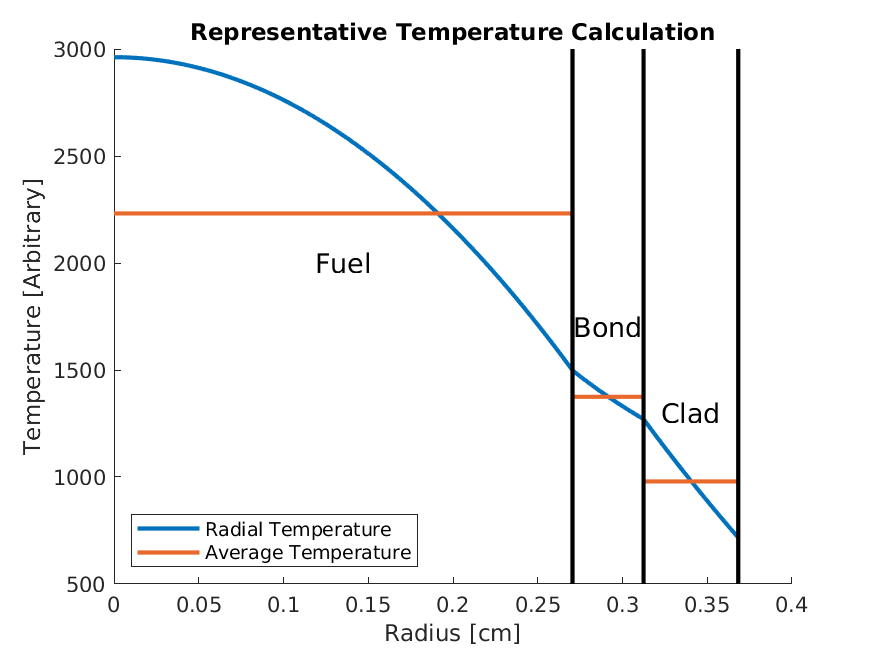
\includegraphics[width=0.7\textwidth]{radial_temp_plot}
      \caption{Radial Temperatures for Typical Reactor Conditions.}
      \label{fig:radial_temp_plot}
    \end{figure}

  \subsection{Axial Results}
    An exact solution for axial temperatures exists for a given heat generation
    rate and for constant $k_F$. This exact model is compared to a numerical
    model as developed in \sref{sec:axial_convection_model}. For this solution,
    allow
    \begin{equation}
      q'''(z) = q'''_0 \, \sin\left( \frac{\pi \, z}{H}\right)
    \end{equation}
    where $q'''_0$ is dictated by the power of the reactor $Q_{Rx}$. Assume the
    properties in \tref{tab:axial_model_properties} where $H$ is the channel
    height.
    
    \begin{table}
      \caption{System Properties for Axial Model Verification.}
      \label{tab:axial_model_properties}
      \begin{center}
        \begin{tabular}{clc}
          \toprule
          Property & Value \\
          \midrule
          $q'''_0$    & $6.93 \times 10^9$ &
            \units{$\frac{\text{W}}{\text{m}^3}$} \\
          $\mdot$     & 68.56  &\units{$\frac{\text{kg}}{\text{s}}$} \\
          %$k_F$       & 36.82  &\units{$\frac{\text{W}}{\text{m K}}$} \\
          $T_{inlet}$ & 400.   &\units{K} \\
          $h_{in}$    & 246.62 &\units{$\frac{\text{kJ}}{\text{kg}}$} \\
          $H$         & 1.2    &\units{m} \\
          $R_F$       & 0.27051 & \units{cm} \\
          $N_{rod}$   & 271     \\
          \bottomrule
        \end{tabular}
      \end{center}
    \end{table}
    
    First, convert $q'''(z)$ to $q'(z)$ as
    \begin{equation}
      \label{eq:qprime}
      q'(z) = \pi \, R_F^2 \, N_{rod} \, q'''(z)
    \end{equation}
    and as a result,
    \begin{equation}
      q'_0 = \pi \, R_F^2 \, N_{rod} \, q'''_0.
    \end{equation}
    Begin with the calculation of $h(x)$ using 
    \eref{eq:continuous_heat_balance}. Then,
    \begin{align}
      h(z) &= h_{in} + \frac{1}{\mdot} 
        \int_0^z q'_0 \sin\left(\frac{\pi z'}{H}\right)\;dz' \\
      &= h_{in} + \frac{q'_0}{\mdot} \frac{H}{\pi}
        \left(1 - \cos\left(\frac{\pi \, z}{H}\right)\right)
    \end{align}
    and $T_{\infty}(z) = T(h(z))$ given by a sodium state relationship.

    Note that the discretization error is only due to the approximation of the
    integral in \eref{eq:continuous_heat_balance} with the summation in 
    \eref{eq:heat_balance}. Given the linear heat generation rate in
    \eref{eq:qprime}, the total heat generated in node $i$ located 
    ${z \in [z_{i-1/2},z_{i+1/2}]}$ is 
    \begin{equation}
      q_i = q'_0 \frac{H}{\pi} \left( \cos\left(\frac{\pi \,
      z_{i-1/2}}{H}\right) - \cos\left(\frac{\pi \, z_{i+1/2}}{H}\right)
      \right)
    \end{equation}
    and then $h_{i+1/2}$ is computed using \eref{eq:heat_balance}.
    
    The result of the axial discretization is an error in the bulk coolant
    temperature axially, $T_{\infty}(z)$. All subsequent calculations of surface
    temperatures and average temperatures are analytical and exact to within the
    approximations made (e.g. constant thermal conductivity). Therefore, the
    error is only computed as it relates to $T_{\infty}(z)$. Analytic and
    modeled results are shown in \fref{fig:axial_difference_plot} as well as the
    difference between the two results. The error for the nodaliztion selected 
    is less than 10 \units{K}. Average axial temperatures for the discrete model 
    are shown in \fref{fig:axial_temp_plot}.

    \begin{figure}
      \centering
      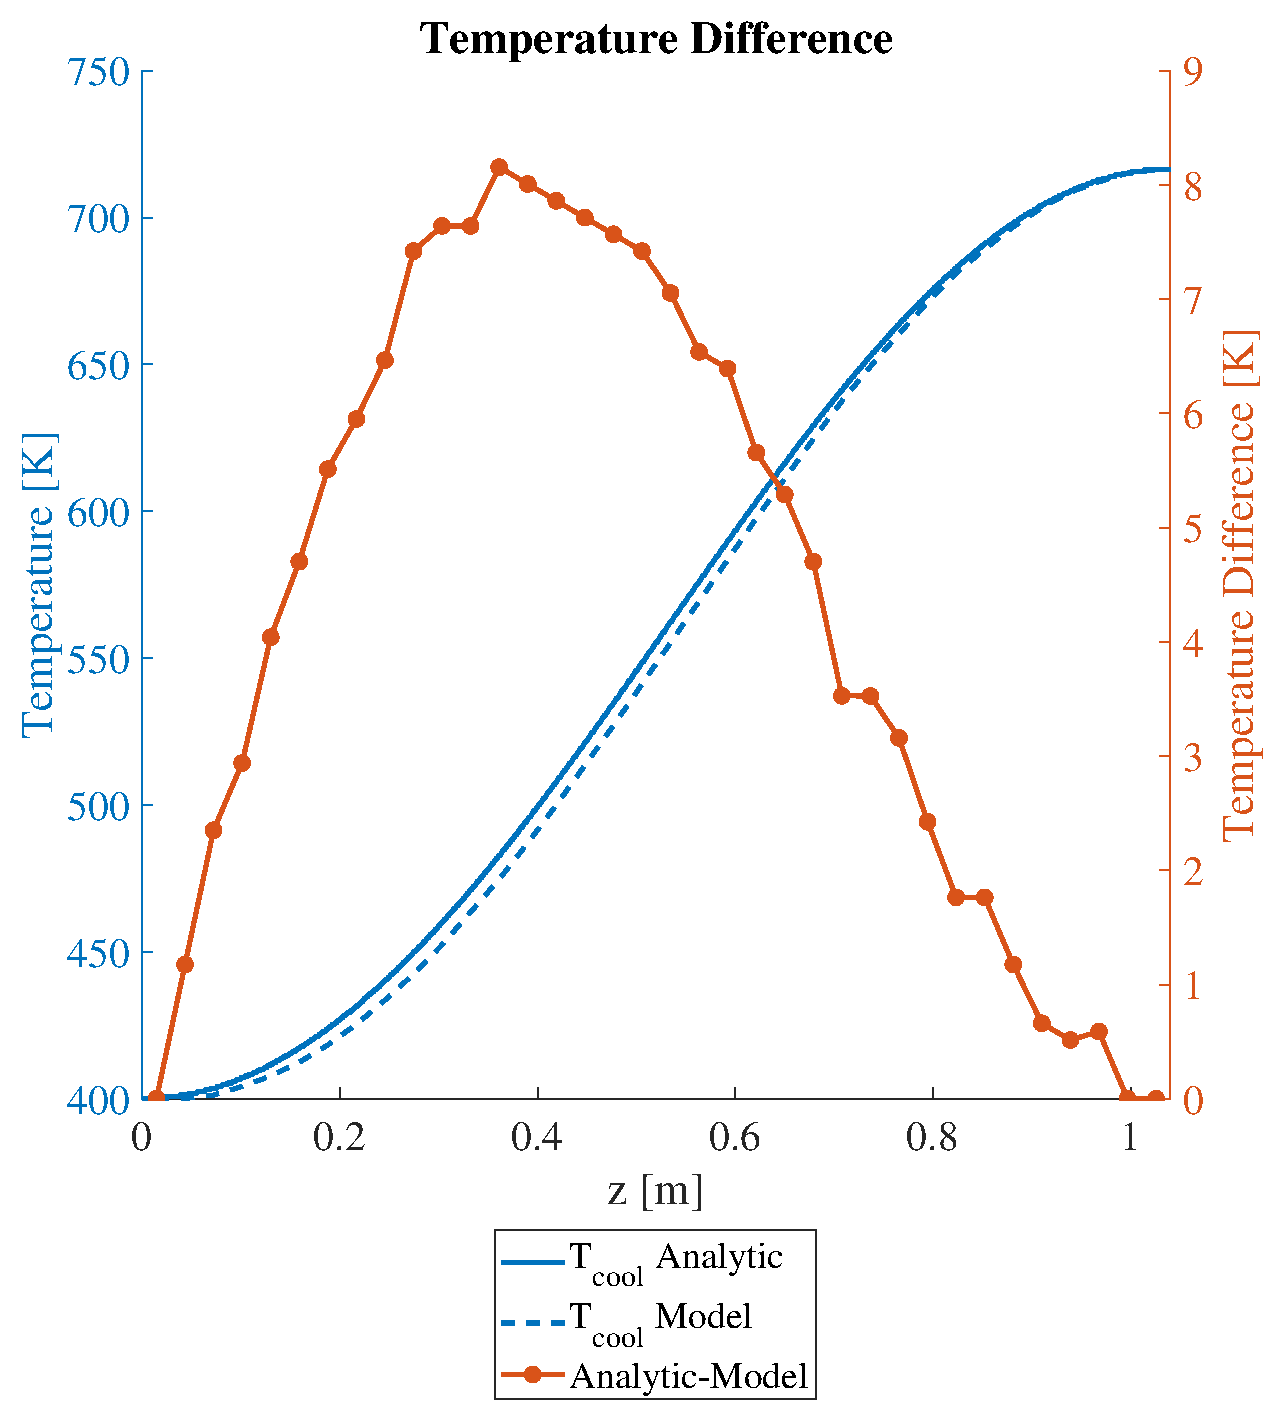
\includegraphics[width=0.8\textwidth]{axial_difference_plot}
      \caption{Difference Between Analytic and Modeled Axial Temperatures.}
      \label{fig:axial_difference_plot}
    \end{figure}

    \begin{figure}
      \centering
      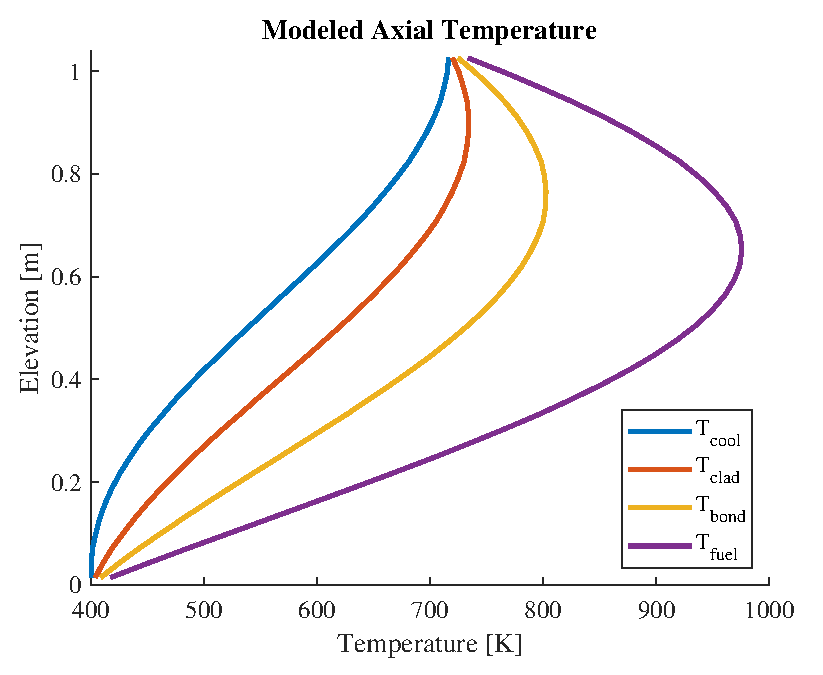
\includegraphics[width=0.7\textwidth]{axial_temp_plot}
      \caption{Average Axial Temperatures for Model Reactor Conditions.}
      \label{fig:axial_temp_plot}
    \end{figure}
